\chapter{Modélisation de la chaîne}
\label{chap:measurement-chain-modelisation}

Reprenant le schéma bloc des étapes clé des techniques de mesure de la figure \ref{fig:flowChartTechMes_chaine_de_mesure}, nous souhaiterions aborder le traitement des mesures. Toutefois nos connaissances de la chaîne de mesure sont encore insuffisantes: nous devons maintenant comprendre comment modéliser la chaîne de mesure afin d'avoir les outils et informations nécessaires aux traitements mathématiques qui vont suivre.

Pour résoudre le problème de la mesure, à savoir retrouver la valeur du mesurande à partir de la sortie du capteur, il faut inverser la fonction mathématique $F(X)$ liant le mesurande à la sortie. La difficulté vient du fait que F(X) est mal définie: du bruit s'ajoute au signal de sortie, les grandeurs d'influence modifient la fonction, les tolérances de fabrication conduisent à une fonction réelle légèrement différente de la fonction nominale. De plus les lois physiques qui régissent le capteur et la chaîne de mesure peuvent conduire à une expression mathématique complexe de la fonction.

\section{Approximations mathématiques}

Nous avons vu au chapitre \ref{chap:introduction} que les approximations mathématiques pouvaient être faites au travers de modèles de formes mathématiques diverses: linéaire, polynomiale ou découlant directement de la loi physique exploitée dans le capteur. Pour la suite de l'analyse, \textbf{nous ne considérerons ici que le cas linéaire.}

\section{Incertitudes}

Le modèle linéaire est une droite, ne passant pas nécessairement par l'origine, approchant au mieux la caractéristique de la chaîne de mesure:

\begin{center}
\fbox{\textbf{Y = G X  + Of}}
\end{center}

Cette équation fait intervenir les deux paramètres G et Of, caractéristiques de la chaîne.

\begin{definition}
	Le gain $G$ est la pente de la caractéristique entrée-sortie.
\end{definition}

\begin{definition}
	Le décalage $Of$ est l'ordonnée à l'origine du modèle linéaire (de l'anglais \emph{offset}).
\end{definition}

Il est fondamental de ne jamais oublier qu'il ne s'agit là que d'une approximation de la courbe de réponse (forme de la réponse pas tout à fait droite, tolérances de fabrication), et de plus que cette approximation est variable dans le temps, en raison des grandeurs d'influence (vieillissement, température, ...) ou des conditions d'utilisation (effet de charge, perturbations,...). Le fabricant nous indique les valeurs nominales du gain et du décalage $G_{nom}$ et $Of_{nom}$.
On résout le problème de mesure sur la base de ces valeurs nominales, et l'on obtient alors une estimation $X_{m}$ de la grandeur d'entrée $X$:

\begin{center}
\fbox{
\begin{minipage}{0.96\textwidth}
\textbf{\textit{Déf}. Erreur absolue (e) :}
Écart entre la valeur mesurée et la vraie valeur 	$e = X_{m} - X$
\newline
\newline
\textbf{\textit{Déf}. Erreur relative ($\epsilon$) : }
\text{Quotient entre erreur absolue et vraie valeur  }	$\epsilon = \frac{e}{X}  \cong \frac{e}{X_{m}}$
\end{minipage}
}
\end{center}

Pour analyser l'erreur, il faut tenir compte des écarts entre la courbe réelle et son approximation linéaire dans les conditions de mesure, ainsi que du fait que cette approximation diffère légèrement de la droite nominale. Nous écrivons donc une nouvelle expression de la sortie Y
\begin{equation}
Y = G_{reel}X + Of_{reel} + L(X,t)
\end{equation}
où $G_{reel}$ et $Of_{reel}$ représentent le modèle linéaire actuel, tenant compte des grandeurs d'influence et effets de charge. $L(X,t)$ représente l'écart entre la courbe et la droite du modèle actuel, ainsi que le bruit ajouté à la sortie. On ne connaît jamais ces trois termes, mais un étalonnage dans des conditions données des grandeurs d'influence permet au fabricant de spécifier les écarts maximum. Exprimons l'erreur:
\begin{gather}
e = X_m - X =  Y - \frac{Of_{nom}}{G_{nom}} - X = \frac{G_{reel}X + Of_{reel} + L -Of_{nom}}{G_{nom}} - X\\
e = X \cdot(\frac{G_{reel}}{G_{nom}}   - 1) +  \frac{Of_{reel} - Of_{nom}}{G_{nom}}   +  \frac{L}{G_{nom}}
\end{gather}
c.-à-d.
\begin{equation}
e = X \cdot \alpha  + D + NL
\end{equation}
On constate alors que l'erreur est la somme de trois termes. Les deux premiers expriment des erreurs systématiques fonctions des grandeurs d'influence (dérive du modèle linéaire par rapport aux valeurs nominales), le troisième peut être assimilé à une erreur aléatoire.
\begin{center}
\fbox{
\begin{minipage}{0.95\textwidth}
\textbf{\textit{Déf}. Erreur de gain  ($\alpha$) :}\\
Erreur relative du gain de la chaîne: Gréel - GnomGnom  .  Correspond à une rotation de la courbe autour de l'origine. Provoque une erreur systématique proportionnelle au mesurande (calculable seulement si l'on connaît toutes les grandeurs d'influence)\\
\\
\textbf{\textit{Déf}. Erreur de décalage (D) :}\\
Erreur absolue à l'origine: Ofréel - OfnomGnom  . Correspond à une translation verticale de la courbe de réponse. Provoque une erreur systématique constante, indépendante de X (calculable seulement si l'on connaît toutes les grandeurs d'influence)\\
\\
\textbf{\textit{Déf}. Erreur de non-linéarité (NL)}\\
Écart entre la droite du modèle actuel et la courbe réelle de réponse. Fonction du mesurande, si bien qu'on la considère comme une grandeur aléatoire.
\end{minipage}
}
\end{center}
Le fabricant indique l'incertitude de la chaîne ou d'un appareil en combinant ces trois erreurs et le bruit interne.

\begin{center}
\fbox{
\begin{minipage}{0.96\textwidth}
\textbf{\textit{Déf}. Incertitude de mesure :	}
Valeur limite que peut prendre l'erreur (en valeur absolue), avec un certain degré de confiance, en général 99 \%. En d'autres termes, si l'on a spécifié une incertitude I, la valeur absolue de l'erreur e sera dans 99 \% des cas inférieure à I : 	|e| < I 	(99 fois sur 100)
\end{minipage}
}
\end{center}

\begin{figure}
\centering
\includegraphics[height=8cm]{assets/figures/3_1_Non_Linearite.PNG}
\caption{Non-linéarité.}
\label{fig:Non-linéarité}
\end{figure}
La spécification de l'incertitude comprend deux termes, pour tenir compte du fait que l'une des composantes est proportionnelle à X. L'erreur de gain est toujours spécifiée sous forme d'une valeur relative $\alpha$ (en \%, \textperthousand ~ ou ppm, soit des facteurs de $10^{-2}, 10^{-3}, ou 10^{-6}$), alors que l'effet global du décalage, des non-linéarités et du bruit interne est spécifié comme un terme indépendant de X, soit sous forme absolue B (unités de X, ou unités d'affichage: divisions sur un écran analogique, digit sur un affichage numérique), soit sous forme relative $\beta$ par rapport à une grandeur caractéristique de la chaîne: gamme de mesure, étendue de mesure, ou pleine échelle.
\begin{equation}
I = \alpha \cdot \text{lect} + B \cdot digit = \alpha \cdot \text{lect} + \beta \cdot \text{gamme}
\end{equation}

\begin{figure}[h]
\centering
\includegraphics[height=10.7cm]{assets/figures/incertitudes.pdf}
\caption{Évolution des incertitudes absolues et relatives en fonction du mesurande.}
\label{fig:incertitudes_absolues_et_relatives}
\end{figure}

La figure \ref{fig:incertitudes_absolues_et_relatives} nous montre que l'incertitude absolue est maximum en haut de gamme, alors que l'incertitude relative tend vers l'infini lorsque X tend vers zéro. Lorsqu'on doit évaluer l'imprécision d'un système de mesure, on le fera soit en estimant l'incertitude absolue en haut de gamme, soit l'incertitude relative en bas de gamme (recherche du pire des cas).

Lorsqu'on fait l'évaluation d'un mesurande qui évolue dans une plage de variation donnée, on cherchera avantageusement à relativiser l'incertitude par rapport à la pleine échelle (PE, en anglais FS pour "Full Scale") de cette variation, et de l'exprimer alors en \%(PE) ou \%(FS). Par exemple, l'information fournie par un capteur de pression qui évolue entre 950 et 1100 mbar permet bien de savoir à quel endroit se trouve la pression le long des 150mbar d'évolution possible. Dans ce cas c'est donc bien la pleine échelle qui nous intéressera comme référence.

Par ailleurs, lorsqu'on cherche à faire une mesure d'une grandeur avec un appareil donné, on remarquera souvent que la valeur B augmente quasi proportionnellement avec la gamme alors que $\alpha$ reste assez stable quelle que soit la gamme. Ainsi, pour de bonnes mesures il est indispensable de choisir la plus petite gamme de mesure possible. On aura ainsi un B minimal.

\section{Calibrage et étalonnage}

Sur de nombreuses chaînes de mesure on dispose d'un amplificateur avec lequel on peut ajuster le gain et le décalage. On est alors amené, au moment de la mise en service de la chaîne, à ajuster cet amplificateur, de manière à obtenir la réponse la plus proche que possible de l'idéal (modèle nominal). C'est ce qu'on appelle le calibrage (en anglais: gauging ou calibration), opération qui vise à annuler les erreurs de gain et de décalage. Une autre opération consiste, sans modifier la chaîne, à déterminer son modèle réel, et l'écart entre le modèle réel et le modèle nominal. C'est l'opération d'étalonnage(en anglais: calibration). Cette opération peut être faite dans un but de correction ou de vérification. Dans ce dernier cas, la chaîne est acceptée si elle se trouve dans les tolérances, ou rejetée sinon. Dans le cas de la correction, alors un moteur de correction sera mis en oeuvre par l'utilisateur de la chaîne de mesure pour exploiter non pas le modèle nominal, mais le modèle réel mesuré.
On notera que la terminologie française est cette fois plus précise que la terminologie anglaise où la distinction entre calibrage et étalonnage ne se fait pas. Ce flou se retrouve en français lorsqu'on utilise l'anglicisme "calibration", alors que ce terme s'applique normalement à des méthodes de datation en dendrochronologie.
\begin{center}
\fbox{
\begin{minipage}{0.96\textwidth}
\textbf{\textit{Déf}. Étalonnage :	}
Ensemble des opérations permettant de déterminer le modèle réel de la chaîne de mesure, et donc de déterminer les erreurs de mesure par rapport au modèle nominal.\\

\textbf{\textit{Déf}. Calibrage :	}
Ensemble des opérations d'ajustage des différents réglages de la chaîne, pour l'amener à un fonctionnement aussi juste que possible, c'est-à-dire aussi proche que possible du modèle nominal.
\end{minipage}
}
\end{center}

Dans ces opérations, il faut imposer à l'entrée de la chaîne une valeur connue du mesurande, et observer la sortie de la chaîne. Quatre situations peuvent se présenter :
\begin{enumerate}[a)]
\item Dans de très rares cas, on dispose d'un moyen d'imposer une valeur exacte (par exemple une tension nulle au moyen d'un court-circuit).
\item Parfois on dispose d'un étalon (par exemple 0 \degree C au moyen d'un mélange d'eau et de glace fondante), et la valeur imposée n'est connue qu'avec une certaine incertitude.
\item Dans la majorité des cas, il faut mesurer la grandeur d'entrée avec des instruments de précision, et  régler la valeur désirée, ce qui conduit également à une incertitude sur cette valeur.
\item Enfin il peut être impossible d'imposer une grandeur d'entrée connue et stable (par exemple 1200 \degree C), on procède alors par simulation du capteur en générant la grandeur électrique qu'il est censé produire (résistance, charge électrique, tension, etc.) sous l'effet de la grandeur physique désirée; l'incertitude provient alors d'une part de la qualité des générateurs, d'autre part de celle du capteur (on simule un capteur parfait, alors que le capteur réel ne l'est pas).
\end{enumerate}
L'idéal recherché généralement est de connaître le mesurande avec une incertitude inférieure à $1/10$ de l'incertitude de la chaîne à étalonner ou à calibrer.

\subsection{Calibrage}

Pour ajuster le gain et le décalage, il suffit de faire passer la réponse par deux points connus. Si ces 2 points sont choisis arbitrairement, il est évident que les deux réglages seront dépendants l'un de l'autre, et qu'il faudra procéder par approximations successives: imposer $X_{0}$, ajuster le décalage de la chaîne pour $Y_{0} = G_{nom} \cdot X_{0} + Of_{nom}$; puis imposer $X_{max}$ et ajuster le gain pour $Y_{max} = G_{nom} \cdot X_{max} + Of_{nom}$; revenir à $X_{0}$ et corriger le décalage ...etc.

Si l'on connaît la construction et les signaux à l'intérieur de la chaîne, alors on peut choisir $X_{0}$ de telle manière que le signal interne soit nul. Dans ce cas le gain n'influence pas l'ajustage du décalage, et l'opération peut se faire en deux étapes seulement.

L'ajustage des potentiomètres ne sera jamais exact : les bruits internes dans la chaîne et  la résolution du potentiomètre conduisent à une erreur d'affichage résiduelle.

Ainsi on applique généralement le mesurande X et on effectue plusieurs mesures Y qui permettent de déterminer une moyenne de la valeur appliquée et une moyenne de la valeur mesurée, ainsi que les minima et maxima. On détermine ainsi un rectangle d'incertitude. On établit ensuite un rectangle d'incertitude centré sur la valeur moyenne en maximisant les écarts autour de la valeur moyenne. Les valeurs moyennes permettront de déterminer le modèle réel.

\begin{figure}
\centering
\includegraphics[width=12cm]{assets/figures/3_3_explications.PNG}
\caption{Un point de mesure, avec les incertitudes sur la valeur appliquée X et sur la valeur mesurée Y.}
\label{fig:3_3_explications}
\end{figure}

\begin{figure}
\centering
\includegraphics[width=12cm]{assets/figures/3_3a_reel_versus_nominal.PNG}
\caption{Mesure après calibrage: modèles nominal et réel.}
\label{fig:3_3a_reel_versus_nominal}
\end{figure}

\begin{figure}
\centering
\includegraphics[width=12cm]{assets/figures/3_3b_incertitude_de_offset.PNG}
\caption{Mesure après calibrage: incertitude sur l'offset.}
\label{fig:3_3b_incertitude_de_offset}
\end{figure}

\begin{figure}
\centering
\includegraphics[width=12cm]{assets/figures/3_3c_incertitude_de_gain.PNG}
\caption{Mesure après calibrage: incertitude sur le gain.}
\label{fig:3_3b_incertitude_de_gain}
\end{figure}

En résumé, le calibrage consiste à :

\begin{center}
\fbox{
\begin{minipage}{0.96\textwidth}
\textbf{ }
\begin{itemize}
\item Imposer un mesurande $X_0$ nul correspondant au zéro de mesure, et ajuster le décalage de la chaîne pour obtenir l'offset du modèle nominal ; le zéro est le point sur lequel le gain n'a pas d'effet.
\item Imposer la valeur maximum $X_{max}$ de mesure et ajuster le gain (span) de la chaîne pour obtenir la valeur correspondante selon le modèle nominal.
\item Déterminer les incertitudes sur les valeurs ajustées et en déduire les incertitudes de calibrage:	$D_{c} = \Delta X_{o} + \frac{\Delta Y_{o}}{G} $ et
$\alpha _{c} = \frac{D_{c} + \Delta X_{max} + \frac{\Delta Y_{max}}{G}}{X_{max} -X_{o}} $
\end{itemize}
\end{minipage}
}
\end{center}

Après une opération de calibrage, on peut généralement considérer que les erreurs de gain et de décalage ont été annulées. Par conséquent, pour les mêmes valeurs des grandeurs d'influence (raisonnablement quelques minutes à quelques heures après le calibrage) seules interviennent les erreurs de non-linéarité et le bruit interne. C'est pourquoi un calibrage préalable est très souvent utilisé dans les procédures de mesure. Dans ce cas on utilisera comme référence le modèle nominal.

Dans certains cas, lorsque les moyens de réglage ne nous permettent pas de nous rapprocher suffisamment du modèle nominal ou lorsqu'on cherche à améliorer la précision, alors on choisira comme référence le modèle réel obtenu par étalonnage, mesuré après calibrage. Dans ce dernier cas, alors les valeurs $\Delta X_{o}$ et $\Delta Y_{o}$ ainsi que $\Delta X_{max}$ et $\Delta Y_{max}$ seront généralement établies autour des valeurs moyennes de $\Delta X$ et $\Delta Y$.

Lorsqu'il n'est pas possible ou pas souhaitable d'appliquer un mesurande nul, l'évaluation des incertitudes suivra le même principe que ci-dessus, mais il faudra tenir compte du fait que chacun des points $X_{min}$ et $X_{max}$ influencent la réponse à $X_{0}$, et donc la valeur du décalage. Les relations pour $D_{c}$ et $\alpha_{c}$ ne sont alors pas valables.

\subsection{Étalonnage}

Ici, il faut établir un tableau de mesure, couvrant toute l'étendue de mesure. Manuellement on se contente d'une dizaine de mesures répartie entre le minimum et le maximum. Lorsqu'on utilise un système d'acquisition, on recherche un beaucoup plus grand nombre de mesures, couvrant plusieurs cycles sur l'étendue de mesure, de manière à permettre la mise en évidence de phénomènes éventuels tels que l'hystérèse, la répétabilité ou le bruit de mesure.

Pour chaque couple mesuré $(X(i), Y(i))$, on peut déterminer l'erreur
\[
e(i) = X_m(i) - X(i) = \frac{Y(i) - Of_{nom}}{G_{nom}}   -X(i)
\]
mais ceci ne nous permet pas de bien séparer les composantes de l'erreur.

Il convient donc de déterminer le modèle actuel de la chaîne, c'est-à-dire $G_{réel}$ et $Of_{réel}$, après quoi on pourra séparer les composantes d'erreur (gain, décalage, non-linéarité et bruit). La manière de définir la droite de réponse influence quelque peu les résultats, si bien qu'il est indispensable d'utiliser une définition commune, si l'on veut comparer les résultats (par exemple avec les spécifications individuelles des composants de la chaîne). On utilise généralement deux méthodes de choix de cette droite:
\begin{center}
\fbox{
\begin{minipage}{0.96\textwidth}
\textbf{Droite par les extrêmes (End points linearity) :}
la droite passe par deux points de la courbe de réponse réelle (en général le zéro et la pleine échelle, ou encore les deux extrémités du domaine de mesure).\\

\textbf{Meilleure droite (Best fit linearity) :}
C'est la droite de régression linéaire, elle minimise la somme des carrés des écarts entre la courbe de réponse réelle et la droite ainsi définie.
\end{minipage}
}
\end{center}

Le gain réel $G_{reel}$ est la pente de la droite ainsi choisie. Le décalage réel $D_{reel}$ est l'ordonnée à l'origine de la droite. Pour chaque couple mesuré $(X(i),Y(i))$ on détermine l'écart entre la valeur mesurée et la droite $\Delta = Y(i) - [G_{reel}\cdot X(i) + Of_{reel}]$. Cet écart est une combinaison de l'erreur de non-linéarité et du bruit. Pour une utilisation immédiate après le calibrage, cet écart représente l'erreur résiduelle du montage, et on en spécifie la limite maximum en valeur absolue, dans l'unité du mesurande, ce qui revient à diviser $max{|\Delta|}$ par le gain de la chaîne:
\[
	NL+Bruit = \frac{max{|\Delta|}}{G_{reel}}
\]
Une séparation du bruit et de la non-linéarité n'est généralement pas nécessaire.
Les erreurs de gain et de décalage du modèle réel par rapport au modèle nominal se calculent en comparant $G_{reel}$ et $Of_{reel}$ avec $G_nom$ et $Of_nom$ :

\[\alpha =  \frac{G_{reel}-G_{nom}}{G_{nom}}	 \]
\[D =  \frac{Of_{reel}-Of_{nom}}{G_{nom}} \]

Dans certains cas on sera amené à établir les incertitudes de gain et de décalage du modèle réel par rapport à lui-même, dues à des instabilités constatées sur l'affichage et à des difficultés d'appliquer un mesurande parfaitement stable. Dans ce cas on procédera comme au point précédent pour l'établissement des incertitudes de calibrage.

\subsection{Auto calibrage }
Les avantages apportés par un calibrage juste avant une série de mesures sont tels qu'il devient indispensable de le réaliser pour compenser les effets des grandeurs d'influence si l'on veut atteindre une haute précision. C'est pourquoi de nombreux équipements de précision incorporent une séquence automatique de calibrage (ou au moins d'ajustage du zéro = auto zéro) à intervalles réguliers ou même avant chaque mesure. Ce calibrage peut se faire de manière analogique ou entièrement numérique.
Pour permettre un auto calibrage, il suffit d'insérer un commutateur permettant de déconnecter l'entrée normale de mesure pour la remplacer par les étalons correspondants à $X_0$ et à $X_{max}$. La séquence de travail lors du calibrage est semblable à la séquence manuelle, si ce n'est qu'il faut mémoriser les valeurs de correction. Ensuite, il faut soit agir sur les réglages matériels, soit utiliser un moteur de correction, qui n'est en fait rien d'autre qu'un calculateur. Si ce calculateur se trouve dans la chaîne de mesure et que celle-ci fournit une sortie numérique ainsi calibrée, alors on a bien un auto calibrage. Toutefois dans certains cas la chaîne de mesure fournit d'une part le signal sans correction, d'autre part les paramètres de correction. Dans ce dernier cas, on parlera alors d'auto étalonnage.

\section{Compensation des erreurs systématiques}

Au lieu d'un auto calibrage, il est parfois plus efficace de faire une compensation directe d'une erreur systématique, s'il est possible d'identifier son influence. Un cas typique se présente dans les capteurs de pression intégrés où la température est l'influence prépondérante ; souvent c'est également l'influence de la tension d'alimentation qu'il faut pouvoir compenser.

\subsection{Compensation linéaire }
L'identification consiste à déterminer les coefficients d'influence agissant sur le gain et le décalage de la chaîne. Généralement on se contente de déterminer $G_r$ et $Of_r$ aux deux valeurs extrêmes d'utilisation. En faisant l'hypothèse que l'évolution du gain et celle du décalage sont linéairement dépendantes de la grandeur d'influence, on définit les coefficients d'influence :

\begin{center}
\fbox{
\begin{minipage}{0.96\textwidth}
\textbf{\textit{Déf}. Coefficient d'influence sur le gain : }
variation relative du gain par unité de la grandeur d'influence. Représente l'erreur de gain additionnelle due à la grandeur d'influence $Z_i : d\alpha / dZ_i = (dG_r/G_r)/dZ_i$ (proportionnelle à X : exprimée en$ \%/unité de Z_i$)
\\
\\
\textbf{\textit{Déf}. Coefficient d'influence sur le décalage :}
variation d'offset par unité de la grandeur d'influence. Représente l'erreur de décalage additionnelle due à la grandeur d'influence $Z_i$ : \\
\begin{equation}
{dD}{dZ_i} = \frac{(dOf_r/G_r)}{dZ_i}\text{ }[\frac{unites de X}{unites de Z_i}]
\end{equation}
\end{minipage}
}
\end{center}

Pour effectuer la correction, il suffit alors de mesurer $Z_i$ (chaîne auxiliaire), d'en déduire la variation par rapport à la valeur de $Z_i$ au moment du calibrage, et de multiplier les coefficients d'influence par cet écart pour connaître la variation de gain ou de décalage par rapport au calibrage.

À titre d'exemple, prenons un capteur de pression intégré. La grandeur d'influence est la température T. On commence par étalonner le capteur aux deux températures extrêmes d'utilisation, ici environ 25 et 60 \degre C. Une telle mesure est présentée sur le graphique ci-dessous.

\begin{figure}
\centering
\includegraphics[height=10cm]{assets/figures/3_5_identification_reponse_en_temperature.PNG}
\caption{ Identification de la réponse du capteur aux températures extrêmes.}
\label{fig:IdentificationTemperature}
\end{figure}

On en déduit les coefficients d'influence, en prenant les valeurs exactes mesurées à une température de calibrage, ici 25.8 \degre C :
Gain:
\[
\frac{d\alpha}{dT} = \frac{dGr/Gr}{dT} = \frac{(96.324-103.968)/103.968}{ (61.1-25.8)} =\]
\begin{equation}
= \frac{-0.0735}{35.3} = -0.002083 = -0.21 \% \text{/ \degre C}
\end{equation}

Décalage:
\begin{equation}
\frac{dD}{dT} = \frac{(dOfr/Gr)}{dT} = \frac{(2.724-3.979)/103.968}{(61.1-25.8)} =
 \frac{-0.012 bar}{ 35.3 \text{\degre C}} = -0.34 \text{mbar/ \degre C}
\end{equation}

Par conséquent, si l'on mesure alors que la température est de 38.0 \degre C, nous avons un écart de température de (38.0 - 25.8) = 12.2 \degre C et les erreurs additionnelles de gain et de décalage par rapport aux valeurs de calibrage (gain 103.968 mV/bar et offset 3.979 mV) seront de :

$d\alpha = -0.002083 \cdot 12.2 = -0.0254 = -2.54 \% lect $
\\
$dD = -0.34 m \cdot 12.2 = - 4.148 mbar $

Pour corriger les indications, il est généralement plus simple de calculer le gain et l'offset actuels avant de traduire la sortie (mV) en valeurs de pression :

$G(38 \text{\degre C}) = G(25.8 \text{\degre C}) (1 + d \alpha) = 103.968(1-0.0254) = 101.327 mV/bar $
\\
\\
$Of(38 \text{\degre C}) = Of(25.8 \text{\degre C}) + G(25.8 \text{\degre C}) \cdot dD = 3.979 - 4.148 \cdot 10-3 \cdot 103.968 = 3.548 mV$
\\

Ainsi une sortie de 89 mV correspond à une pression de (89-3.548) / 101.327 = 0.843 bar.

Sans correction, avec les valeurs de calibrage on obtient 0.731 bar : on sous-évalue la pression, car la température introduit un décalage négatif de -4.2 mbar ainsi qu'une erreur de gain négative de -2.54\% de 731 mbar soit -15.6 mbar, et donc un total de -19.8 mbar.

\subsection{Moteur de correction mathématiques}

La puissance de calcul des microprocesseurs incorporés aux capteurs dits \textless\textless\ intelligents \ \textgreater\textgreater permet d'envisager des corrections bien plus efficaces, qui sont maintenant incorporées dans les profils d'utilisation de ces capteurs (réseau de terrain).
À titre d'exemple, la norme IEEE-1451 / Smart Transducers, définit une fonction multi - variables, de type polynomial, et décomposable par segments :

\begin{equation}
\displaystyle\sum_{i=0}^{D(1)}
\displaystyle\sum_{j=0}^{D(2)} \text{...}
\displaystyle\sum_{p=0}^{D(n)} C_{i,j,...,p} [X_1-H_1]^i[X_2-H_2]^j \text{...} [X_n-H_n]^p
\end{equation}

Le calcul de correction ci-dessus représente une somme polynomiale de n variables, dont on peut choisir indépendamment les degrés de chaque variable. Dans le cas de la compensation linéaire de température, nous aurions $X_1$ = sortie en mV du capteur de pression, $X_2$ = sortie du capteur de température, les degrés D(1) et D(2) seraient tous deux égaux à 1 (linéaire), et la formule permet de calculer la valeur de pression. Par conséquent la formule de calcul devient :
\begin{equation}
P_m =C_{00} + C_{10} \cdot (X_1-H_1)+C_{01} \cdot (X_2-H_2) + C_{11}\cdot(X_1-H_1) \cdot (X_2-H_2)
\end{equation}

\begin{equation*}
= C_{00} + C_{01} \cdot X_2 + X_1 \cdot (C_{10} + C_{11} \cdot X_2)  \text{ si les termes $H_1$ et $H_2$ sont nuls }
\end{equation*}

On voit bien qu'ainsi on a bien un décalage $(C_{00} + C_{01} \cdot X_2)$ dépendant de $X_2=T$ et un gain $(C_{10} + C_{11} \cdot X_2)$ également dépendant de T. Par contre cette méthode permet des corrections bien plus évoluées (polynômes et compensation de plusieurs grandeurs d'influence).

Pour de grands domaines ou pour de fortes non-linéarités, afin d'éviter des polynômes de degré trop élevé, la norme prévoit de segmenter la réponse selon les valeurs des différentes variables, et d'exploiter un ensemble de paramètres de faible degré dans chaque segment, comme illustré dans la figure ci-dessous.

\begin{figure}
\centering
\includegraphics[height=6cm]{assets/figures/3_6_Correction_a_2_variables_segementees.PNG}
\caption{Correction à deux variables segmentées.}
\label{fig:Correction_a_2_variables_segementees}
\end{figure}

A chaque élément de surface (désigné par "Cell") correspond un ensemble de paramètres $C_{ij}$ et $H_x$ permettant d'approcher la surface réelle en minimisant le nombre total de paramètres à mémoriser.

\section{Mesures répétées}

Lors de mesures répétées de la même valeur du mesurande X, on constate que les résultats ne sont pas toujours parfaitement ceux qu'on attend, et ne sont pas identiques. Une analyse statistique des résultats de mesure permettra d'établir une valeur moyenne $\mu$ de tous les résultats ainsi qu'un écart-type $\sigma$. Les mesures sont en général réparties autour de la moyenne selon une distribution gaussienne caractérisée par cet écart-type. Ainsi la moyenne constitue la partie systématique de l'erreur appelée aussi le biais, alors que l'écart-type représente sa composante aléatoire.

\newpage
On a donc :
\begin{itemize}
\item X, le mesurande
\item La moyenne des mesures $\mu$
\item L'erreur de biais $\beta :  \beta = \mu - X$  [unité de X], erreur systématique
\item L'exactitude ou la justesse, termes utilisés pour caractériser l'erreur systématique
\item L'écart-type $\sigma$ sert à quantifier l'erreur aléatoire
\item La répétabilité ou la fidélité, termes utilisés pour caractériser l'erreur aléatoire
\end{itemize}

\begin{equation}
\mu = \lim\limits_{N \to \infty} \frac{1}{N} \sum_{i=1}^N x_i
\end{equation}

\begin{equation}
\sigma = \lim\limits_{N \to \infty} \sqrt{\frac{1}{N}\sum_{i=1}^N (x_i-\mu)^2}
\end{equation}

\begin{figure}
\centering
\includegraphics[height=7cm]{assets/figures/3_7_Exemple_de_mesures_repetees_N_fois.PNG}
\caption{Exemple de mesures répétées N fois, où N >100 pour être significatif.}
\label{fig:Exemple_de_mesures_repetees_N_fois}
\end{figure}

\begin{figure}
\centering
\includegraphics[height=7cm]{assets/figures/3_8_distinction_entre_repetabiite_et_justesse.PNG}
\caption{distinction entre répétabilité et justesse.}
\label{fig:distinction_entre_repetabiite_et_justesse}
\end{figure}

\begin{figure}
\centering
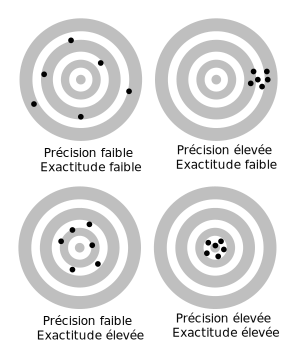
\includegraphics[height=7cm]{assets/figures/juste-fidèle-précis.pdf}
\caption{Autre représentation des notions de justesse et fidélité.}
\label{fig:juste_fidele_precis}
\end{figure}

L'écart-type sert à mesurer la dispersion d'un ensemble de données. Plus il est faible, plus les valeurs sont regroupées autour de la moyenne. Par exemple pour la répartition des notes d'une classe, plus l'écart type est faible, plus la classe est homogène. ¿ l'inverse, s'il est plus important, les notes sont moins resserrées. Dans le cas d'une notation de 0 à 20, l'écart-type minimal est 0 (notes toutes identiques), et peut valoir jusqu'à 10 si la moitié de la classe a 0/20 et l'autre moitié 20/20.

En sciences, il est fréquent de considérer que les valeurs se répartissent selon une courbe de Gauss. Dans le cas des sciences sociales, par exemple, la moyenne $\mu$ et l'écart-type $\sigma$ permettent de déterminer un intervalle dans lequel on trouve une majorité de la population. En effet, si la moyenne est $\mu$ et l'écart type est $\sigma$, on trouve 95 \% de la population dans l'intervalle $[ \mu - 1.96 \sigma ; \mu + 1.96 \sigma ]$ et on trouve 68.2 \% de la population dans l'intervalle $[ \mu - \sigma ; \mu + \sigma ]$.

L'écart-type est aussi utilisé pour construire un intervalle de confiance attribuable à un échantillon. Si l'on se réfère à la figure ci-contre, on voit qu'un $\sigma$ d'écart de part et d'autre de la valeur moyenne recouvre 68,2\% de la distribution, deux $\sigma$ d'écart $(13.6+34.1+34.1+13.6 =) 95.4\%$, 3 $\sigma$ d'écart $(2.1+13.6+34.1+34.1+13.6+2.1 =) 99.6\%$ et ainsi de suite... C'est l'usage notamment en physique des particules, où la détection d'évènements est quantifiée en nombre de sigmas, et où un résultat notamment est considéré comme significatif par l'obtention de 5 $\sigma$, représentant une probabilité d'erreur inférieure à 0,00003\% (niveau de confiance de plus de 99.99997\%).

En pratique, on considère que :
\begin{itemize}

\item $1 * \sigma \rightarrow 68\% $
\item $2 * \sigma \rightarrow 95\% $
\item $3 * \sigma \rightarrow 99.7\%$

\end{itemize}


\begin{figure}
\centering
\includegraphics[height=7cm]{assets/figures/3_9_Loi_normale_et_intervale_de_confiance.PNG}
\caption{Loi normale et intervalle de confiance.}
\label{fig:3_9_Loi_normale_et_intervale_de_confiance}
\end{figure}

\section{Exercices }

\subsection{Exercice: Incertitudes des appareils }
Spécifications:\\
\\
\textbf{HP34401A}: spécifié pour 1 an, $23 \pm 5 \degree C$, en (\%lect+ \%gamme) et jusqu'à 20\% de dépassement de gamme\\
\\
\begin{tabular}{l c c}
\hline
gamme: 	& 100.0000 mV	& 0.0050 + 0.0035 \\
		& 1.000000 V	& 0.0040 + 0.0007 \\
    	& 10.00000 V	& 0.0035 + 0.0005 \\
		& 100.0000 V	& 0.0045 + 0.0006 \\
		& 1000.000 V	& 0.0045 + 0.0010 \\
\hline
\end{tabular}
\\
\\
\textbf{Prema} 6000:spécifs pour 1 an, $23 \pm 5 \degree C$, en (\% of reading + \% of full scale)
	Full scale : 1'999'999 (sauf gamme 1000 V : 1'000'000)
\\
\begin{tabular}{lcc}
\hline
range & $\pm$ 0.2 V & 0.006 + 0.0007 \\
	& $\pm$ 2 V	& 0.005 + 0.0005 \\
	& $\pm$ 20 V	& 0.005 + 0.0006 \\
	& $\pm$ 200 V	& 0.005 + 0.0006 \\
	& $\pm$ 1000 V	& 0.006 + 0.0005 \\
\hline
\end{tabular}
\\
\\
\textbf{APPA-98}: spécifié pour 2 ans, $23 \pm 5 \degree C$ et moins de 75\% humidité relative, en (\% reading + number of digits)
\\
\begin{tabular}{lcl}
\hline
	Range	& Resolution	& Accuracy \\
	200 mV	& 100 $\mu$V	& | \\
	2 V	& 1 mV	& | \\
	20 V	& 10 mV	& |  $\pm$ (0.5 \%rdg + 1 dgt) \\
	200 V	& 100 mV	& | \\
	1000 V	& 1 V	& | \\
\hline
\end{tabular}
\\

\begin{enumerate}
\item Quelles sont les incertitudes absolues et relatives si on mesure 2.2 V avec HP34401A ?
\item Quelles sont les incertitudes absolues et relatives si on mesure 2.2 V avec APPA-98 ?
\item Quelle est l'incertitude relative maximum si on mesure entre 10 et 250 mV avec HP34401A ?
\item Quelle est l'incertitude relative maximum si on mesure entre 10 et 250 mV avec Prema6000 ?
\item Quelle est l'incertitude absolue maximum si l'on mesure entre 30 et 500 V avec APPA-98 ?
\item Représenter les incertitudes relatives du HP34401A et du Prema6000 pour un domaine de 10mV à 1000V (utilisez une échelle Log pour l'axe X des tensions).
\end{enumerate}
NB: la pleine échelle définie pour le PREMA n'est pas la définition habituelle qui dit que la pleine échelle est la différence entre les valeurs min et max. On aurait alors attendu pour le PREMA une pleine échelle égale au double de la gamme.

\subsection{Exercice: Calibrage d'une chaîne}
a)	Une chaîne de mesure de température doit être utilisée pour la régulation de température d'une enceinte, autour de 60 $\degree$ C. On désire qu'elle nous indique l'erreur (température actuelle moins consigne de 60 $\degree$ C). Le calibrage est réalisé ainsi: \\
i)	on place le capteur dans un bain à 60 $\pm$ 0.35 $\degree$ C, et on ajuste le décalage pour un affichage nominal de 0.00. On constate que les indications oscillent entre -0.03 et + 0.08. \\
ii)	on place le capteur dans un bain à 70 $\pm$ 0.5 $\degree$ C, et on ajuste le gain pour un affichage nominal de 10.00. On constate que les indications oscillent entre 9.88 et 10.09. \\  ~ \\
Quelles sont les incertitudes de gain et de décalage dues à ce calibrage ? \\

b)	Une chaîne de mesure doit indiquer l'épaisseur d'une feuille plastic (capteur capacitif sans contact, basé sur la variation de la constante diélectrique). Le calibrage s'effectue comme suit: \\
i)	Pas de feuille dans le capteur, on ajuste le décalage et on obtient un affichage stable de 000. \\
ii)	On place une feuille étalon d'épaisseur 0.500  $\pm$  0.005 mm dans le capteur, et on ajuste le gain pour un affichage nominal de 500. Malheureusement le potentiomètre ne permet pas l'ajustage exact et on doit se contenter d'un affichage oscillant entre 497 et 499. \\~ \\
Quelles sont les incertitudes de calibrage de cette chaîne ? \\

c)	Une chaîne de mesure de la hauteur du liquide contenu dans un réservoir utilise la pression relative à la base de ce réservoir (P = $\rho\,gh$ où h est la hauteur du liquide dans le réservoir). Pour le calibrage on procède comme suit: \\
i)	Réservoir vide, on ajuste le décalage pour un affichage de 0000  $\pm$  0001 \\
ii)	On remplit le réservoir, on mesure une hauteur h = 10.00 $\pm$ 0.02 m, ainsi que la densité du liquide  $\rho$ = 0.800  $\pm$  0.006 kg/dm3, et on ajuste l'affichage à 1000  $\pm$  0003 \\ ~ \\
Quelles sont les incertitudes de calibrage (indication: n'oubliez pas que la chaîne est sensible à la pression et non directement à la hauteur du liquide)? \\

d)	On a calibré un capteur de pression relative (=différence de pression par rapport à l'atmosphère) de la manière suivante : pression appliquée par une pompe dans la tuyauterie du capteur avec une vanne de détente, mesure de la pression appliquée par la différence de hauteur de mercure dans un tube en U, ouvert sur l'atmosphère, lecture de la sortie dans un PC. La réponse nominale est 0 à +2 bar, 0 à +20'000digit (1 bar = 100kPa). \\
i)	Vanne ouverte (= pression atmosphérique), ajustage de l'offset pour une valeur nominale de 0, on obtient un affichage stable de 00'000digit. \\
ii)	Vanne fermée, on agit sur la pompe jusqu'à une hauteur de mercure de 148.5 $\pm$ 0.2cm dans le tube en U. On calcule alors la pression appliquée $P=\rho\,gh = 13.6\times10^3 \text{ kg/m}^3 * 9.81\text {m/s}^2 * 1.485\text{ m}=198.12276\text{ kPa} = 1.98123\text{ bar}$. On ajuste donc le gain pour obtenir un affichage nominal de 19'812.3 digit, et obtient un affichage oscillant entre 19'810 et 19'814. \\ ~\\
Quelles sont les incertitudes de calibrage ?

\subsection{Exercice: Linéarité}

a)On a mesuré la réponse d'un capteur de force à $23 \degree C$ (réponse idéale : $0-100N \Leftrightarrow 0-20 mV$):\\
~
\\
\begin{tabular}{|l|l|l|l|l|l|l|l|l|l|l|l|}
\hline
F [N]	& 0	& 10	& 20	& 30	& 40	& 50	& 60	& 70	& 80	& 90	& 100 \\
\hline
U [mV]	& 0.50	& 2.49	& 4.46	& 6.41	& 8.34	& 10.25	& 12.14	& 14.01	& 15.86	& 17.69	& 19.5 \\
\hline
\end{tabular}
\\

Déterminez l'offset réel en [mV], le gain réel en [mV/N], les erreurs de décalage [N], de gain [\%lect] et l'incertitude de non-linéarité en [N] et en [\%(PE)] de ce montage par les deux méthodes :
\begin{enumerate}
\item Choix de la droite de référence par les extrémités de la courbe de réponse
\item Choix de la "meilleure droite"	 ...
\end{enumerate}
~\\

b)	L'étalonnage d'une chaîne de mesure de couple, gamme 0 à 100 mNm, sortie 4 à 20 mA, a donné: \\
~
\\
\begin{tabular}{|l|l|l|l|l|l|l|l|l|l|l|l|}
\hline
\footnotesize C [mNm]	& 0	& 10	& 20	& 30	& 40	& 50	& 60	& 70	& 80	& 90	& 100 \\
\hline

\footnotesize I [mA]	& \footnotesize  3.960	& \footnotesize  5.564	& \footnotesize  7.192	& \footnotesize  8.800	& \footnotesize  10.443	& \footnotesize  12.063	& \footnotesize  13.677	& \footnotesize  15.315	& \footnotesize  16.926	& \footnotesize  18.550	& \footnotesize  20.160 \\
\hline
\end{tabular}
\\

L'équation nominale de cette chaîne vaut donc $I = 4 [mA] + 0.16 [\frac{mA}{mNm}]  \cdot C [mNm]$.

Quelles sont les erreurs de gain et de décalage ainsi que l'incertitude de non-linéraité + bruit dans les 2 cas suivants:
\begin{enumerate}
\item Choix de la droite de référence par les extrémités de la courbe de réponse
\item Choix de la "meilleure droite"	 ...
\end{enumerate}

\subsection{Exercice: Auto-Calibrage d'une chaîne}

a)	Pour réaliser l'auto calibrage d'un canal de mesure de courant (nominal 0-20 mA, code numériques 0-2000 digits), on procède comme suit:
\begin{itemize}
\item ouverture du circuit de mesure par un interrupteur (donc courant nul), mémorisation du code obtenu :  $N_0=2$ (stable)
\item Fermeture d'un interrupteur reliant une source de tension de référence ($U_g = 10.000V \pm 0.005V$) au circuit de mesure à travers une résistance de $R_g = 500 \Omega \pm 0.1\%$ (la borne de mesure étant supposée travailler à potentiel nul, le courant nominal ainsi imposé est de 20mA). On mémorise alors le code moyen obtenu sur 10 mesures : $N_1 = 2018.3$, alors que les codes max et min sont 2021 et 2015.
\item Les mesures seront ensuite corrigées à l'aide de $N_0$ et $N_1$ pour obtenir :
	\begin{itemize}\itemsep1pt
	\renewcommand{\labelitemi}{$\bullet$}
	\item i) une valeur numérique corrigée ;
	\item ii) une valeur dans l'unité du mesurande ;
	\end{itemize}
\end{itemize}
NB : si ces corrections sont faites à l'extérieur de la chaîne de mesure, alors on parlera d'auto étalonnage.
Quelles sont les fonctions mathématiques de correction et quelles sont les incertitudes de calibrage ?\\

b)	Pour programmer l'auto calibrage d'une chaîne de mesure de température dont le capteur (PT100 : $R(T)=100 \Omega (1+0.00385T)$ a une interchangeabilité de 0.2 $\degree$ C + 0.1\%lecture, on a inséré des interrupteurs programmables permettant de déconnecter le capteur et de le remplacer soit par une résistance de$ 100 \Omega \pm 0.1 \Omega$, soit par une résistance de $138.5 \Omega \pm 0.14 \Omega$. La séquence d'auto calibrage est la suivante :
\begin{itemize}
\item Capteur remplacé par la résistance de $100 \Omega$, on mémorise la moyenne de 100 conversions: on trouve $M_0=1985.65$, toutes les conversions sont soit 1985, soit 1986.
\item Capteur remplacé par la résistance de $138.5 \Omega$. On mémorise la moyenne de 100 conversions: $M_1=2825.45$, conversion maximum 2827, minimum 2824.
\item Pour les mesures, on ne fait qu'une seule conversion $N_x$, et l'on calcule \\
$T= (N_x - M_0)\frac{100}{M_1 - M_0}$
\end{itemize}
Quelles sont les incertitudes de calibrage ? \\

c)	Une chaîne de mesure de pression est constituée d'un capteur-transmetteur avec les spécifications suivantes : gamme -1 à +3 bar, sortie 4 à 20mA, précision 0.5\%lect + 35 mbar ; le courant de sortie est mesuré par une résistance shunt de $10 \Omega \pm 0.012 \Omega$, et un convertisseur gamme $\pm 0.25V$.
Pour programmer l'autocalibrage de cette chaîne, on a inséré des interrupteurs programmables permettant de déconnecter le capteur et de le remplacer soit en laissant le circuit ouvert, soit en reliant une résistance de $490 \Omega \pm 0.2 \Omega$ entre la borne positive du shunt et une source de tension de $+10V \pm 15mV$ (courant nominal de 20 mA). La séquence d'auto calibrage est la suivante :
\begin{itemize}
\item Capteur déconnecté, circuit ouvert on mémorise la moyenne de 100 conversions: on trouve $M_0=-0.73$ digit, toutes les conversions sont soit -1, soit 0 digit.
\item Capteur déconnecté, résistance $490 \Omega$ enclenchée. On mémorise la moyenne de 100 conversions: $M_1=1647.32$, conversion maximum 1646, minimum 1649 digit.
\item Les valeurs de $M_0$ et $M_1$ nous permettent de calculer le gain et l'offset total actuel de la chaîne.
\end{itemize}

Quelles sont les incertitudes de calibrage ?

\subsection{Exercice: Coefficients d'influence}

a)	On a étalonné une chaîne de mesure de position à deux températures:


\begin {center}
\begin{tabular}{lll}
$T_1=25 \degree C$ &	$G_1= 100.3 digit/mm$ &	$Of_1 = 3.4 digit$ \\
$T_2=75 \degree C$ &	$G_2 = 103.5 digit/mm$ &	$Of_2 = -5.8 digit$ \\
\end{tabular}
\end{center}
~\\
\begin{itemize}
\item Déterminer les coefficients d'influence de la température
\item A une température de 40 $\degree$ C, l'indication obtenue est de 1380 digit. Calculer la position correspondante
\end{itemize}
~\\


b)	Une chaîne de mesure du contenu d'un réservoir utilise un capteur de force à jauges de contraintes (pont de Wheatstone à 4 jauges)

\begin{figure}[h!]
\centering
\includegraphics[height=3.7cm]{assets/figures/Exercice_3_5_c.PNG}
\caption{Chaîne de mesure du contenu d'un réservoir.}
\label{fig:Exercice_3_5_c}
\end{figure}

\begin{center}
$R_1 = R_4 = R_0(1 + F \cdot K)$\\
$R_2 = R_3 = R_0(1 - F \cdot K)$\\
\end{center}

Avec K = facteur de jauge et F = force appliquée.\\

On en déduit :	$U_{dm} = U_b ( \frac{ R_4}{R_3+R4} - \frac{R2}{R1+R2} ) = U_b \frac{ Ro(1+KF) -Ro(1-KF)}{2Ro}  = Ub \cdot K \cdot F$ \\
La sortie est donc théoriquement proportionnelle à la force, mais aussi à la tension d'alimentation $U_b$, on parle alors de capteur ratio-métrique : la sortie est une fraction (ratio) de l'alimentation.

On a étalonné la chaîne dans les 3 conditions suivantes :\\

\begin {center}
\begin{tabular}{llll}
$U_b = 5V$ &	$T=25 \degree C$ &	$G_1 = 1015 digit/tonne$ &	$Of_1 = -55 digit$\\
$U_b = 3V$ &	$T=25 \degree C$ &	$G_2 = 609 digit/tonne$ &	$Of_2 = -33 digit$\\
$U_b = 5V$ &	$T=50 \degree C$ &	$G_3 = 1095 digit/tonne$ &	$Of_3 = +12 digit$\\
\end{tabular}
\end{center}
~\\
On suppose les influences indépendantes et linéaires

\begin{itemize}
\item Calculer les coefficients d'influence de la température T et de l'alimentation $U_b$.
\item Calculez le gain et l'offset pour une température $T=30 \degree C$ et une alimentation $U_b=5.5V$
\item Enumérez les coefficients du moteur de correction IEEE1451
\end{itemize}

\subsection{Exercice: Mesures répétées}

Un expérimentateur utilise un capteur de pression différentielle dont on lui a dit que la plage de précision était de $\pm 2\%$, pour une différence de pression de 20 Pa, pour un intervalle de confiance de 95\%. Afin de vérifier cette affirmation, il étalonne le capteur en effectuant 100 mesures de la tension U donnée par le capteur lorsque la pression différentielle est p = 20 Pa (il contrôle cette pression de façon très précise). À partir de son échantillon de 100 mesures, il calcule $\mu = 5V$ et $\sigma = 0.2 V$. Il prétend que le capteur n'est pas aussi précis qu'on le lui avait certifié. Pourquoi?
